%\begin{frame}[fragile]{Mayer Vietoris}
%\begin{figure}
%\begin{tikzpicture}[scale=.5, y=0.6pt, x=.75pt]
%     %row 1
%%     \node[font=\large] at (-50, 800) {$(K, U)$};
%     \draw[fill=afragreen, draw = black,  line width=2]  (47,800) circle (10pt);  
%     \draw[fill=afragreen, draw = black, line width=2]  (117,800) circle (10pt);   
%     \draw[fill=afragreen, draw = black, line width=2]  (190,800) circle (10pt); 
%     \draw[fill=afragreen, draw = black, line width=2]  (261,800) circle (10pt); 
%     \begin{pgfonlayer}{edges}
%            \path[draw=black,fill=black,line width=2] (47,800) -- (117, 800);
%            \path[draw=black,fill=black,line width=2] (117,800) -- (190, 800);
%            \path[draw=black,fill=black,line width=2] (190,800) -- (261, 800);
%      \end{pgfonlayer}      
%      \draw[draw, color=afrablue, fill=none, line join=round,draw opacity=0.978,line width=2] (117, 800) ellipse (100 and 45) node[anchor=north, xshift=-.55in] {$U_0$};
%      \draw[draw, color=afrapurple, fill=none, line join=round,draw opacity=0.978,line width=2] (190, 800) ellipse (100 and 45) node[anchor=north, xshift=.6in] {$U_1$};
%    \end{tikzpicture}
%\caption{Space and Cover}
%\label{fig:space-n-cover}
%\end{figure}
%
%When we have a pair of sets there is another short exact sequence:
%\begin{tikzcd}
% C_*(U_0 \cap U_1) \hspace{1mm} \arrow{r}{x \mapsto (x,x)} & C_*(U_0) \bigoplus C_*(U_1) \hspace{1mm} \arrow{r}{ (x,y) \mapsto x-y} & \hspace{1mm} C_*(U_0 \bigcup U_1) = C_*(X) \\
% \end{tikzcd}
%When you have intersections of 3 or more sets, this becomes the mayer vietoris spectral sequence, with the following initial data:
%\[ E^0_{p,q} = \langle p\text{-chains in a }q\textrm{-way intersection} \rangle \]
%\pause
%We will come back to this. For now, lets take advantage of this covering.
%\end{frame}

%\begin{frame}[fragile]
%\frametitle{Compute homology via subcomplexes}
%\begin{minipage}{.35\textwidth}
%\begin{tikzpicture}[scale=.5, y=0.6pt, x=.75pt]
%     %row 1
%%     \node[font=\large] at (-50, 800) {$(K, U)$};
%     \draw[fill=afragreen, draw = black,  line width=2]  (47,800) circle (10pt);  
%     \draw[fill=afragreen, draw = black, line width=2]  (117,800) circle (10pt);   
%     \draw[fill=afragreen, draw = black, line width=2]  (190,800) circle (10pt); 
%     \draw[fill=afragreen, draw = black, line width=2]  (261,800) circle (10pt); 
%     \begin{pgfonlayer}{edges}
%            \path[draw=black,fill=black,line width=2] (47,800) -- (117, 800);
%            \path[draw=black,fill=black,line width=2] (117,800) -- (190, 800);
%            \path[draw=black,fill=black,line width=2] (190,800) -- (261, 800);
%      \end{pgfonlayer}      
%      \draw[draw, color=afrablue, fill=none, line join=round,draw opacity=0.978,line width=2] (117, 800) ellipse (100 and 45) node[anchor=north, xshift=-.55in] {$U_0$};
%      \draw[draw, color=afrapurple, fill=none, line join=round,draw opacity=0.978,line width=2] (190, 800) ellipse (100 and 45) node[anchor=north, xshift=.6in] {$U_1$};
%    \end{tikzpicture}
%Space and Cover
%\end{minipage}
%\begin{minipage}{.2\textwidth}
%\begin{tikzpicture}[y=1.0pt, x=0.8pt, yscale=-1, scale=.5]
%      \path[draw=black,fill=afragreen, line width=3pt,transform canvas={xshift = 1cm}] (2.57,14.56) -- (1.9450, 33.7380) -- (63.8200,33.5230) -- (63.8200,47.7970) -- (107.5700,25.4260) -- (64.4450,3.0550) -- (63.8200,18.8240) -- (2.5700,14.5620);
%\end{tikzpicture}
%\vspace*{1cm}
%\end{minipage}
%\begin{minipage}{.4\textwidth}
%\begin{tikzpicture}[scale=.5, y=0.6pt, x=.75pt]
%    %disj 0
%    \begin{scope}[shift={(143,80)}]
%    \node[font=\large] at (300, 730) {$K^0 \times \Delta^{0}$};
%     \draw[draw, color=afrablue, fill=none, line join=round,draw opacity=0.978,line width=2] (117, 730) ellipse (100 and 45);
%     \draw[fill=afrablue, draw = black, line width=2]  (47,730) circle (10pt);  
%     \draw[fill=afrablue, draw = black, line width=2]  (117,730) circle (10pt);   
%     \draw[fill=afrablue, draw = black, line width=2]  (190,730) circle (10pt); 
%     \begin{pgfonlayer}{edges}
%            \path[draw=black,fill=black,line width=2] (47,730) -- (117, 730);
%            \path[draw=black,fill=black,line width=2] (117,730) -- (190, 730);
%      \end{pgfonlayer}   
%      \end{scope}
%      %disj  1
%       \begin{scope}[shift={(0,0)}]
%        \node[font=\large] at (380, 680) {$K^1 \times \Delta^{1}$};
%       \draw[draw, color=afrapurple, fill=none, line join=round,draw opacity=0.978,line width=2] (190, 680) ellipse (100 and 45);
%     \draw[fill=afrapurple, draw = black, line width=2]  (117,680) circle (10pt);   
%     \draw[fill=afrapurple, draw = black, line width=2]  (190,680) circle (10pt); 
%      \draw[fill=afrapurple, draw = black, line width=2]  (261,680) circle (10pt); 
%         \begin{pgfonlayer}{edges}
%            \path[draw=black,fill=black,line width=2] (117,680) -- (190, 680);
%            \path[draw=black,fill=black,line width=2] (190,680) -- (261, 680);
%      \end{pgfonlayer}   
%            \end{scope}
%      %blowup edges 
%      \begin{scope}[shift={(143,80)}]
%     \begin{pgfonlayer}{edges}
%            \path[draw=black,fill=black,line width=2] (47,730) -- (47, 600);
%            \path[draw=black,fill=black,line width=2] (117,730) -- (117, 600);
%      \end{pgfonlayer}     
%          \node[font=\large] at (280, 665) {$K^{[1]} \times \Delta^{[1]}$};
%        \begin{pgfonlayer}{quadcell}
%      \draw [fill=afragreen,  preaction={fill, afragreen}, pattern=north west lines, pattern color=black] (47, 600) rectangle (117, 730);
%	\end{pgfonlayer}
%	\end{scope}
%\end{tikzpicture}
%The blowup complex.
%\end{minipage}
%{\color{blue}{Definition:}} \[ K^{U} = \bigcup_{J \in N(U)} U_J \times J \]
%where $U_J = \bigcap_{j \in J} U_j$ and $N(U)$ is the nerve of $U$.
%\pause
%\begin{theorem}[Segal]
%For any closed cover $U$, $K^U$ and $K$ are homotopy equivalent.
%\end{theorem}
%\pause \textbf{Recipe for a parallel \emph{homology} algorithm}
%\end{frame}
%\begin{frame}
\frametitle{Parallel Algorithm}
\begin{figure}[t]
\def\svgwidth{.8\textwidth} 
\input{images/blowup-persistence.pdf_tex}
\end{figure}
\hspace{-.5cm}\textbf{Algorithm:}
\begin{itemize} 
	\item<1->[Step 1:] Compute the homology of each local piece (in parallel)
	\item<2->[Step 2:] Compute the homology with the blowup pieces (in serial)
\end{itemize}
\only<3->{
\hspace{-.5cm} \textbf{Goal:} 
\begin{itemize}
	\item Do most of work Step 1, Do as little as possible in Step 2.
	\item Equivalent to \textit{quickly} generating ``balanced'' and 
		``minimal'' covers.
\end{itemize}
}
\end{frame}

\begin{frame}
\frametitle{Finding Minimum Blowups}
\textbf{Goal:} Quickly generate cover, $\U$, with balanced size and ``minimal''
overlap.  \\
\vspace{.1cm}
\pause
\textbf{Formally:} 
Given $\alpha \in (\frac{1}{n},1)$ find a covering 
$\U = \{ \U_1, \ldots, \U_n \}$ minimizing: 
\[ \frac{\card{K^\U}}{\card{K}} \] \pause 
subject to:  
\[ \max_{i\in[n-1]}{\card{\U_{i}}} \leq \alpha \card{K} \] \pause 
\end{frame}

\begin{frame}
\frametitle{Finding Minimum Blowups} 
\textbf{Bad News:}
\begin{itemize}
\item<1-> $\frac{\card{K^\U}}{\card{K}}$ is \emph{at worst exponential} in
	$\card{U}$ 
\item<2-> We prove finding $\alpha$-balanced Minimal Blowups is
	$\mathsf{NP}$-Hard.
\end{itemize}
\only<3->{\textbf{Good News:}}
\begin{itemize}
\item<3-> Any cover gives us correct results. 
\item<4-> Approximate minimal blowups should still parallelize well.
\item<5-> We provide a heuristic algorithm with:
	\only<6-> {
		\[ \factor < 3 \]
		guaranteed!
	}
\end{itemize}
\end{frame}

	
%%%%%%%%%%%%%%%%%%%%%%%%%%%%%%%%%%
\begin{frame}
\frametitle{Cover Generation Algorithm}
\begin{itemize}
\item \textbf{Input: } Simplicial Complex $K$, and number of cover sets $n$
\item \textbf{Output:} Covering $\U$ into $n$ cover sets.
\end{itemize}
\begin{figure}
\def\svgwidth{.55\textwidth} 
\only<1>{\includesvg{images/algorithm_1}
\caption{Input Complex}}

\only<2>{\includesvg{images/algorithm_2}
\caption{Extract Graph of complex}}

\only<3>{\includesvg{images/algorithm_3}
\caption{Find partition of graph's vertex set (minimize edgecut)}}

\only<4>{\includesvg{images/algorithm_4}
\caption{Find partition (open cover) of complex}}

\only<5>{\includesvg{images/algorithm_5}
\caption{Close the extra set}}

%\only<6->{\includesvg{images/algorithm_6}
%\caption{(Optional) Union last set}}

\end{figure}
\end{frame}

\begin{frame}{Input Datasets}
\begin{itemize}
	\item Connected Cliques ({\multiblob}) $46 \times 10^6$ Dim: $10$
	\item Clique ({\clique}) $1 \times 10^6$ Dim: $19$
	\item Stanford Bunny ({\bunny}) $9.7 \times 10^6$ Dim: $3$
	\item Sphere ({\sphere}) $19 \times 10^6$ Dim: $8$
	\item {\Erdos}-{\Renyi} Random ({\gnp}) $3.6 \times 10^6$ Dim: $4$
\end{itemize}
\begin{figure}
	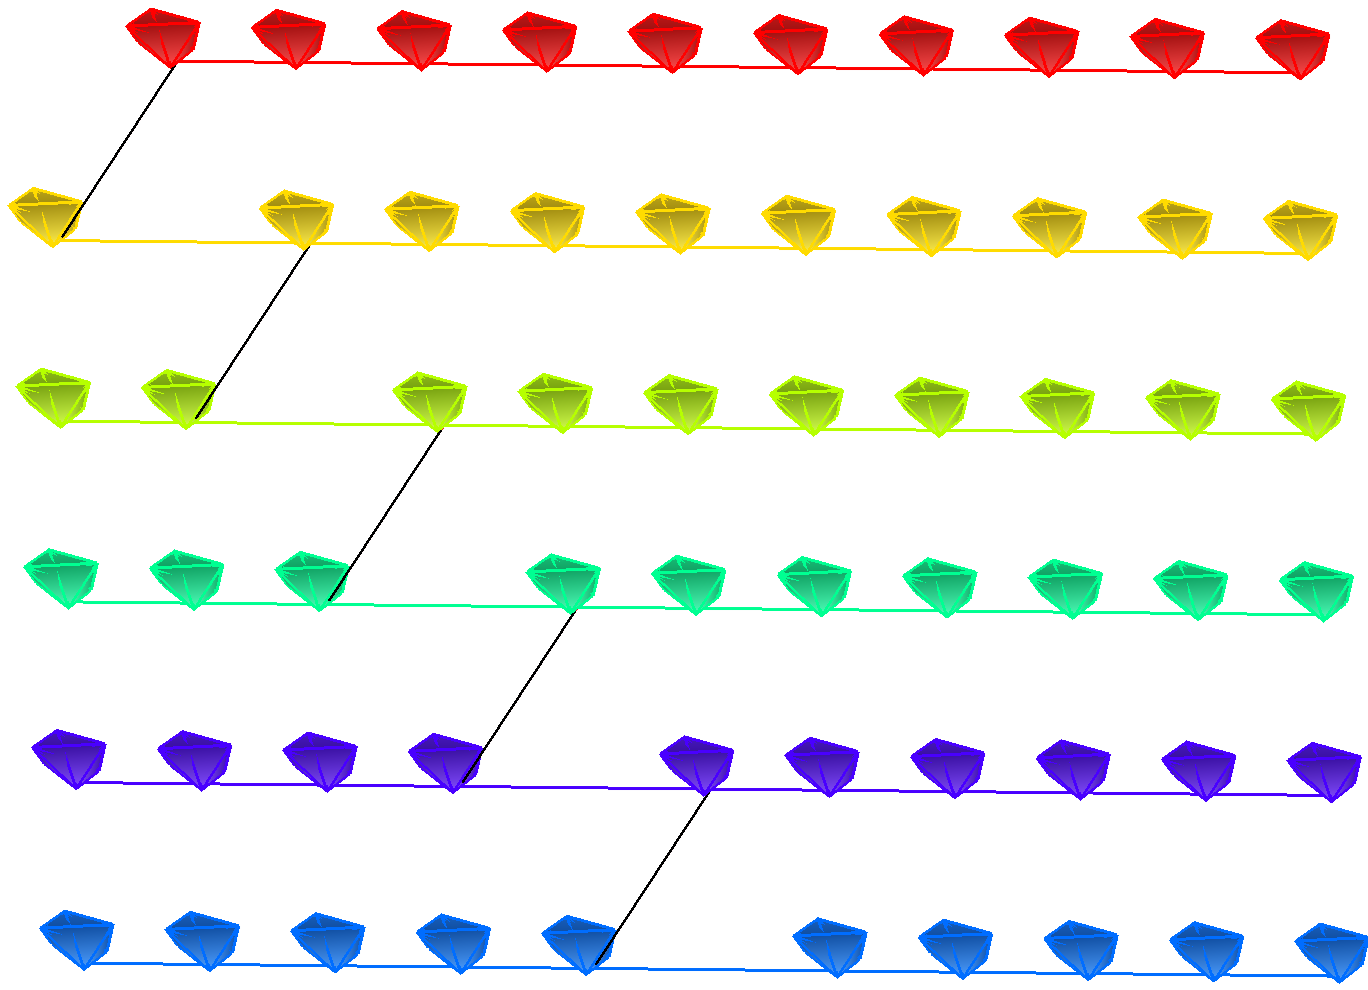
\includegraphics[width=.25\textwidth]{embedding.png}
	\hfill
	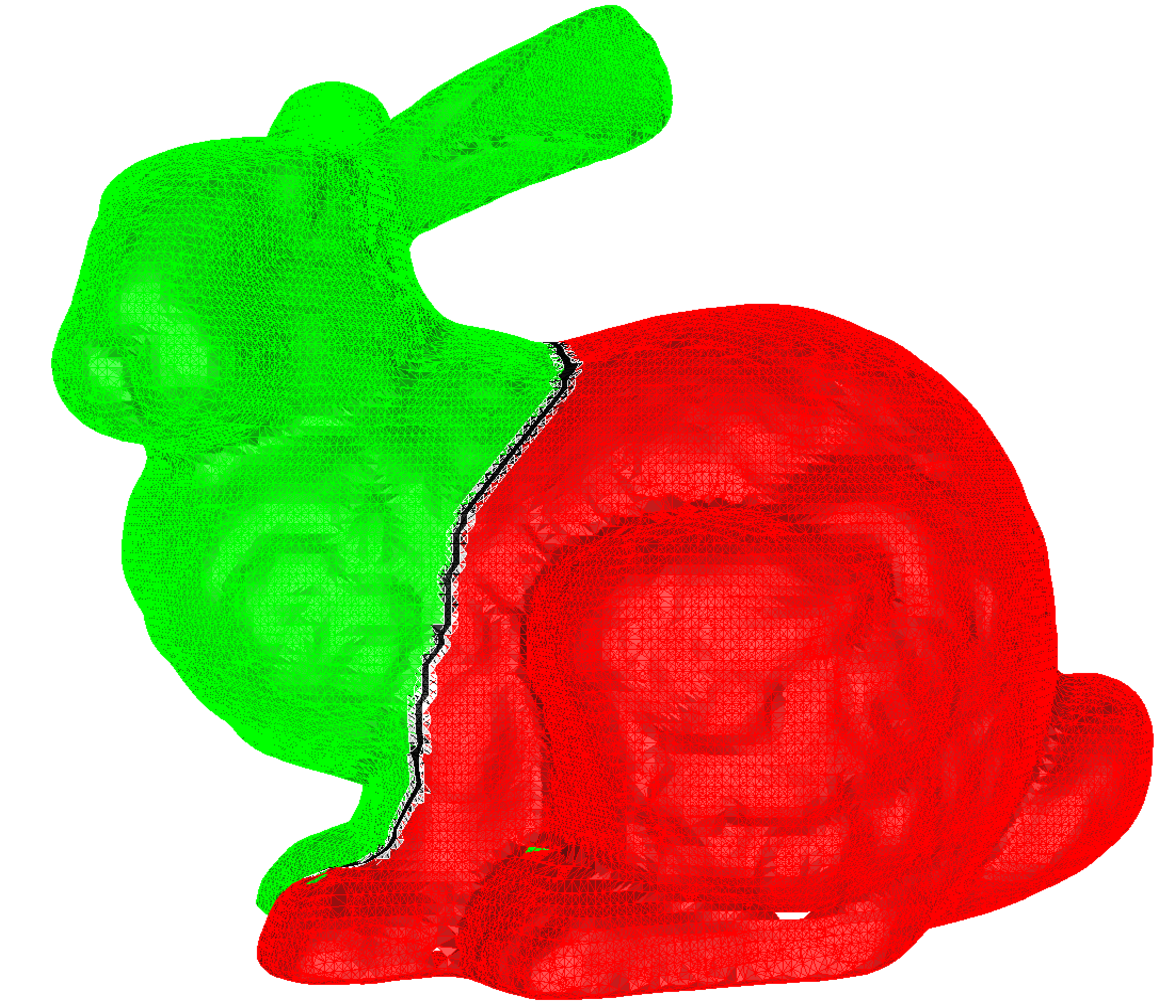
\includegraphics[width=.25\textwidth]{bunny-2.pdf}
	\hfill
	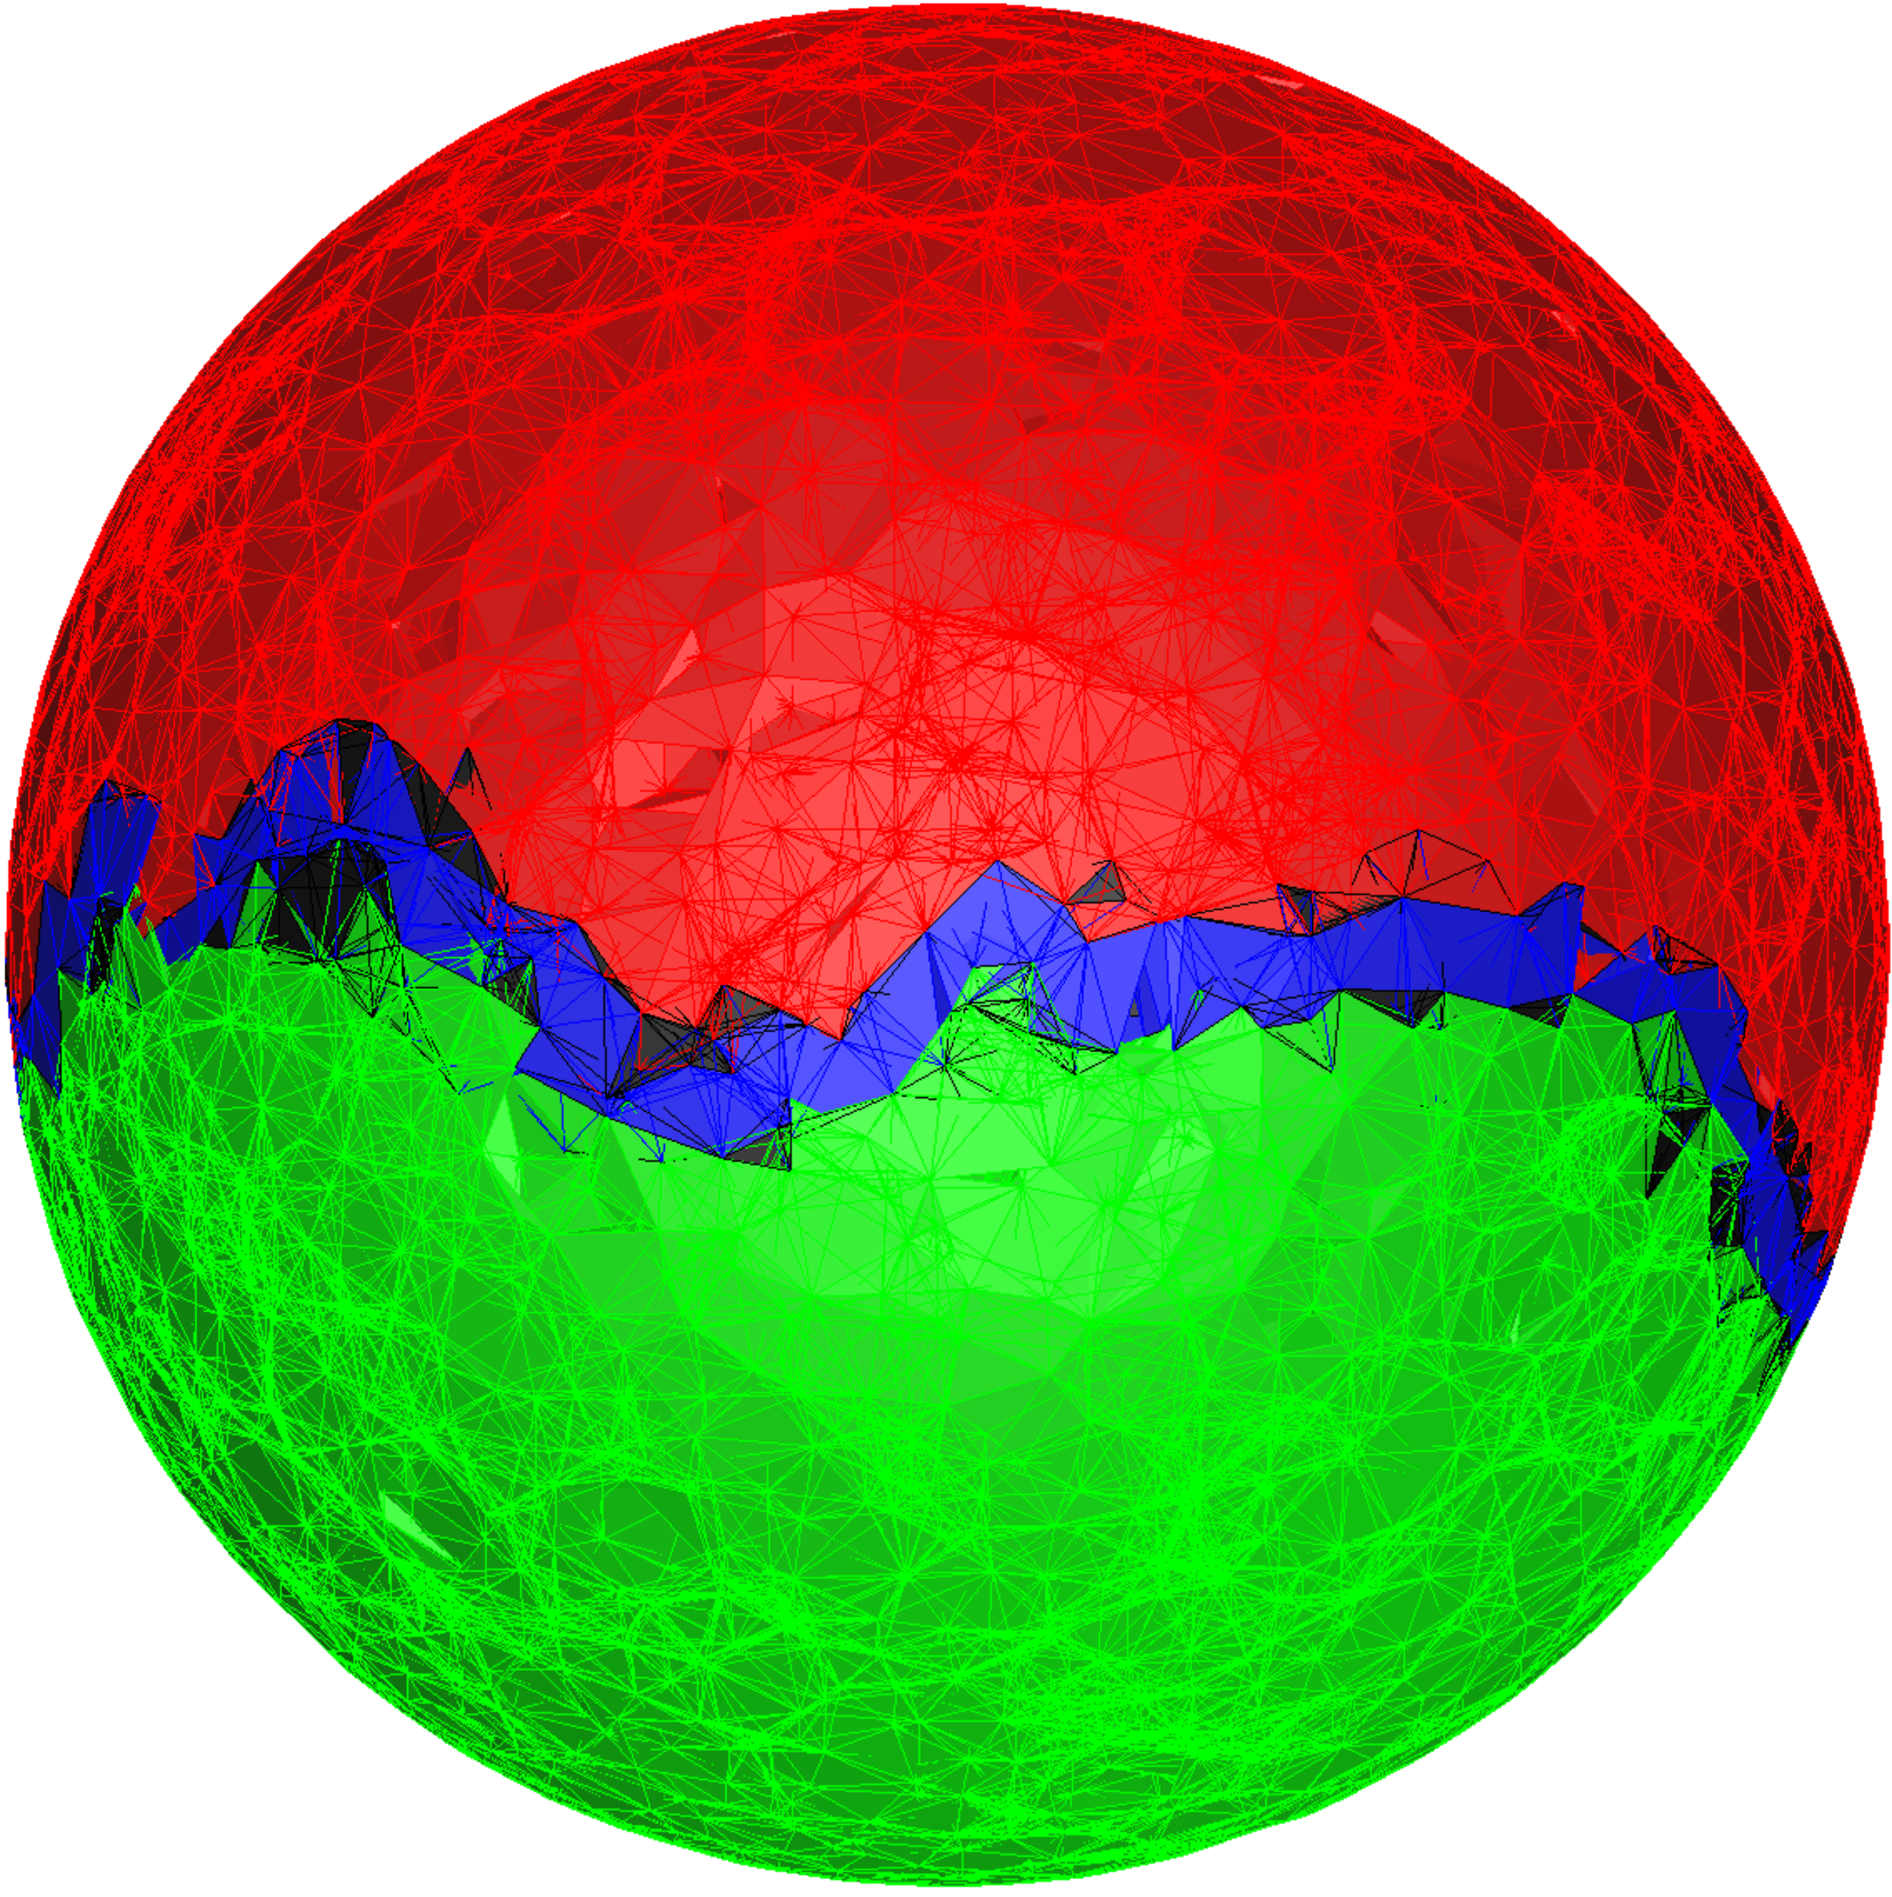
\includegraphics[width=.25\textwidth]{sphere-2.pdf}
\caption{Visualizations of {\multiblob}, {\bunny}, {\sphere}}
\end{figure}
\end{frame}

\begin{frame}
\begin{minipage}{.5\textwidth}
\centering
\begin{figure}
\centering
\begin{tikzpicture}[scale=.525]
\begin{axis}[xlabel=\# of partitions, ylabel={$\hat{\alpha}= \max_i \card{P_i} / \card{\K}$}, legend style={legend pos=north east, font=\small}]
\legend{\multiblob, \bunny, \clique, \gnp, \sphere, ideal}
\addplot table [x=num_partitions, y=graph_balance_ratio, col sep=comma] {pgf-speedup-figs/results/concurrent_homology/clique.11.22720.csv};
\addplot table [x=num_partitions, y=graph_balance_ratio, col sep=comma] {pgf-speedup-figs/results/concurrent_homology/bunny..05.csv};
\addplot table [x=num_partitions, y=graph_balance_ratio, col sep=comma] {pgf-speedup-figs/results/concurrent_homology/clique.20.csv};
\addplot table [x=num_partitions, y=graph_balance_ratio, col sep=comma] {pgf-speedup-figs/results/concurrent_homology/gnp.1250.047.csv};
\addplot table [x=num_partitions, y=graph_balance_ratio, col sep=comma] {pgf-speedup-figs/results/concurrent_homology/sphere.csv};
\addplot[dash pattern=on 4pt off 1pt on 4pt off 4pt, domain=2:10]{1/x};
\end{axis}
\end{tikzpicture}
\caption{Partition Balance Ratio $\hat{\alpha}$}
\end{figure}
\end{minipage}
\begin{minipage}{.5\textwidth}
\begin{figure}
\centering
\begin{tikzpicture}[scale=.525]
%\pgfplotsset{ymax=5}
\begin{axis}[xlabel=\# of partitions, ymax=50000, ylabel={\# of edges}, legend style={legend pos=north west, font=\small}]
\legend{\multiblob, \bunny, \clique, \gnp, \sphere, ideal}
\addplot table [x=num_partitions, skip coords between index={0}{1}, y=edgecut, col sep=comma, ignore chars=']
{pgf-speedup-figs/results/concurrent_homology/clique.11.22720.csv};
\addplot table [x=num_partitions, skip coords between index={0}{1}, y=edgecut, col sep=comma, ignore chars=']
{pgf-speedup-figs/results/concurrent_homology/bunny..05.csv};
\addplot table [x=num_partitions, skip coords between index={0}{1}, y=edgecut, col sep=comma, ignore chars=']
{pgf-speedup-figs/results/concurrent_homology/clique.20.csv};
\addplot table [x=num_partitions, skip coords between index={0}{1}, y=edgecut, col sep=comma, ignore chars=']
{pgf-speedup-figs/results/concurrent_homology/gnp.1250.047.csv};
\addplot table [x=num_partitions, skip coords between index={0}{1}, y=edgecut, col sep=comma, ignore chars=']
{pgf-speedup-figs/results/concurrent_homology/sphere.csv};
\end{axis}
\end{tikzpicture}
\caption{Edgecut}
\end{figure}
\end{minipage}
\begin{minipage}{.5\textwidth}
\centering
\begin{figure}
\begin{tikzpicture}[scale=.525]
\begin{axis}[xlabel=\# of partitions, ylabel={$\alpha = \max_i \card{\C_i} / \card{\K}$}, legend style={legend pos=north east, font=\small},legend style={at={(.95,.55)},anchor=east}]
\legend{\multiblob, \bunny, \clique, \gnp, \sphere, ideal}
\addplot table [x=num_partitions, y=cover_balance_ratio, col sep=comma,skip coords between index={0}{1}] 
{pgf-speedup-figs/results/concurrent_homology/clique.11.22720.csv};
\addplot table [x=num_partitions, y=cover_balance_ratio, col sep=comma, skip coords between index={0}{1}] 
{pgf-speedup-figs/results/concurrent_homology/bunny..05.csv};
\addplot table [x=num_partitions,skip coords between index={0}{1}, y=cover_balance_ratio, col sep=comma] 
{pgf-speedup-figs/results/concurrent_homology/clique.20.csv};
\addplot table [x=num_partitions, skip coords between index={0}{1},y=cover_balance_ratio, col sep=comma] 
{pgf-speedup-figs/results/concurrent_homology/gnp.1250.047.csv};
\addplot table [x=num_partitions, skip coords between index={0}{1},y=cover_balance_ratio, col sep=comma] 
{pgf-speedup-figs/results/concurrent_homology/sphere.csv};
\addplot[dash pattern=on 4pt off 1pt on 4pt off 4pt, domain=2:10]{1/x};
\end{axis}
\end{tikzpicture}
\caption{Balance Ratio for $\C$}
\end{figure}
\end{minipage}
\begin{minipage}{.5\textwidth}
\begin{figure}
\centering
\begin{tikzpicture}[scale=.525]
\begin{axis}[xlabel=\# of partitions, ylabel=$\ratio$, legend style={legend pos=north east, font=\small},legend style={at={(.95,.55)},anchor=east}]
\legend{\multiblob, \bunny, \clique, \gnp, \sphere, worst case}
\addplot table [x=num_partitions, y=blowup_factor, col sep=comma,skip coords between index={0}{1}] 
{pgf-speedup-figs/results/concurrent_homology/clique.11.22720.csv};
\addplot table [x=num_partitions, y=blowup_factor, col sep=comma, skip coords between index={0}{1}] 
{pgf-speedup-figs/results/concurrent_homology/bunny..05.csv};
\addplot table [x=num_partitions,skip coords between index={0}{1}, y=blowup_factor, col sep=comma] 
{pgf-speedup-figs/results/concurrent_homology/clique.20.csv};
\addplot table [x=num_partitions, skip coords between index={0}{1},y=blowup_factor, col sep=comma] 
{pgf-speedup-figs/results/concurrent_homology/gnp.1250.047.csv};
\addplot table [x=num_partitions, skip coords between index={0}{1},y=blowup_factor, col sep=comma] 
{pgf-speedup-figs/results/concurrent_homology/sphere.csv};
\addplot[dash pattern=on 4pt off 1pt on 4pt off 4pt, domain=2:10]{3};
\end{axis}
\end{tikzpicture}
\caption{Blowup Factor}
\label{fig:blowup-factors}
\end{figure}
\end{minipage}
\end{frame}

\begin{frame}
\begin{figure}
\centering
\begin{tikzpicture}[scale=.55]
\begin{semilogyaxis}[
name=plot1,
ymin=.09,
ymax=25,
xmin=0,
xmax=12,
xlabel=\# of  threads, 
title={$Multicore-Homology$},
ylabel= time to reduce boundary matrix (seconds),
minor y tick num={5},
legend style={at = {(.25,.6)}, font=\large}]
%\legend{\multiblob, \bunny, \clique, \gnp, \sphere}
\addplot table [x=num_threads, y=persistence, col sep=comma] {pgf-speedup-figs/results/concurrent_homology/clique.11.22720.csv};
\addplot table [x=num_threads, y=persistence, col sep=comma] {pgf-speedup-figs/results/concurrent_homology/bunny..05.csv};
\addplot table [x=num_threads, y=persistence, col sep=comma] {pgf-speedup-figs/results/concurrent_homology/clique.20.csv};
\addplot table [x=num_threads, y=persistence, col sep=comma] {pgf-speedup-figs/results/concurrent_homology/gnp.1250.047.csv};
\addplot table [x=num_threads, y=persistence, col sep=comma] {pgf-speedup-figs/results/concurrent_homology/sphere.csv};
\end{semilogyaxis}
\begin{semilogyaxis}[
name=plot3,
at=(plot1.below south east), anchor=above north east,
ymin=.09,
ymax=25,
xmin=0,
xmax=12,
xlabel= \# of threads,
title={$Heuristic-MH$},
%ylabel= time to reduce boundary matrix (seconds),
minor y tick num={5},
legend style={at={(1,.55)}, font=\large}]
%\legend{\multiblob, \bunny, \clique, \gnp, \sphere}
\addplot table [x=num_partitions, y=persistence, col sep=comma] {pgf-speedup-figs/results/cover_homology/clique.11.22720.csv};
\addplot table [x=num_partitions, y=persistence, col sep=comma] {pgf-speedup-figs/results/cover_homology/bunny..05.csv};
\addplot table [x=num_partitions, y=persistence, col sep=comma] {pgf-speedup-figs/results/cover_homology/clique.20.csv};
\addplot table [x=num_partitions, y=persistence, col sep=comma] {pgf-speedup-figs/results/cover_homology/gnp.1250.047.csv};
\addplot table [x=num_partitions, y=persistence, col sep=comma] {pgf-speedup-figs/results/cover_homology/sphere.csv};
\end{semilogyaxis}

\begin{semilogyaxis}[
name=plot4,
at=(plot3.right of north east), anchor=left of north west,
ymin=.09,
ymax=25,
xmin=0,
xmax=12,
xlabel= \# of threads, 
title={$Spectral-Sequence$},
minor y tick num={5},
legend style={at={(.95,.525)}, font=\large}]
\legend{\multiblob, \bunny, \clique, \gnp, \sphere}
\addplot table [x=num_partitions, y=persistence, col sep=comma] {pgf-speedup-figs/results/phat_14_ss/clique.11.22720.csv};
\addplot table [x=num_partitions, y=persistence, col sep=comma] {pgf-speedup-figs/results/phat_14_ss/bunny..05.csv};
\addplot table [x=num_partitions, y=persistence, col sep=comma] {pgf-speedup-figs/results/phat_14_ss/clique.20.csv};
\addplot table [x=num_partitions, y=persistence, col sep=comma] {pgf-speedup-figs/results/phat_14_ss/gnp.1250.047.csv};
\addplot table [x=num_partitions,, y=persistence, col sep=comma] {pgf-speedup-figs/results/phat_14_ss/sphere.csv};
\end{semilogyaxis}

\begin{semilogyaxis}[
name=plot2,
at=(plot4.above north west),
anchor = below south west,
ymin=.09,
ymax=25,
xmin=0,
xmax=12,
xlabel=\# of  threads,
title={$Chunk$},
minor y tick num={5},
legend style={at={(.95,.525)}, font=\large}]
%\legend{\multiblob, \bunny, \clique, \gnp, \sphere}
\addplot table [x=num_partitions, y=persistence, col sep=comma] {pgf-speedup-figs/results/phat_14_chunk/clique.11.22720.csv};
\addplot table [x=num_partitions, y=persistence, col sep=comma] {pgf-speedup-figs/results/phat_14_chunk/bunny..05.csv};
\addplot table [x=num_partitions, y=persistence, col sep=comma] {pgf-speedup-figs/results/phat_14_chunk/clique.20.csv};
\addplot table [x=num_partitions, y=persistence, col sep=comma] {pgf-speedup-figs/results/phat_14_chunk/gnp.1250.047.csv};
\addplot table [x=num_partitions,, y=persistence, col sep=comma] {pgf-speedup-figs/results/phat_14_chunk/sphere.csv};
\end{semilogyaxis}
\end{tikzpicture}
\caption{Time to reduce the boundary matrix for each algorithm.}
\label{fig:ctl_vs_phat}
\end{figure}

\end{frame}
%
%\begin{frame}
%\frametitle{Compute \emph{persistent} homology via subcomplexes}
%So far computes homology, but, not persistent homology. 
%\begin{figure}
%\begin{minipage}[t]{.35\textwidth}
%\coverfilt
% \end{minipage}
%\begin{minipage}{.2\textwidth}
%\begin{tikzpicture}[y=1.0pt, x=0.8pt, yscale=-1, scale=.5]
%      \path[draw=black,fill=afragreen, line width=3pt] (2.57,14.56) -- (1.9450, 33.7380) -- (63.8200,33.5230) -- (63.8200,47.7970) -- (107.5700,25.4260) -- (64.4450,3.0550) -- (63.8200,18.8240) -- (2.5700,14.5620);
%\end{tikzpicture}
%\vspace*{1cm}
%\end{minipage}
%\begin{minipage}[t]{.35\textwidth}
%\cover
%\end{minipage}
%\end{figure}
%%second row
%\pause
%\vspace{-1cm}
%\begin{figure}
%\begin{minipage}[t]{.35\textwidth}
%\disjointunion
% \end{minipage}
%\begin{minipage}{.2\textwidth}
%\begin{tikzpicture}[y=1.0pt, x=0.8pt, yscale=-1, scale=.5]
%      \path[draw=black,fill=afragreen, line width=3pt] (2.57,14.56) -- (1.9450, 33.7380) -- (63.8200,33.5230) -- (63.8200,47.7970) -- (107.5700,25.4260) -- (64.4450,3.0550) -- (63.8200,18.8240) -- (2.5700,14.5620);
%\end{tikzpicture}
%\vspace*{1cm}
%\end{minipage}
%\begin{minipage}[t]{.35\textwidth}
%\blowupcomplex
%\end{minipage}
%\end{figure}
%\vspace{-1cm}
%%second row
%\pause
%\begin{figure}
%\begin{minipage}[t]{.35\textwidth}
%\partialblowup
%\end{minipage}
%\begin{minipage}{.2\textwidth}
%\begin{tikzpicture}[y=1.0pt, x=0.8pt, yscale=-1, scale=.5]
%      \path[draw=black,fill=afragreen, line width=3pt] (2.57,14.56) -- (1.9450, 33.7380) -- (63.8200,33.5230) -- (63.8200,47.7970) -- (107.5700,25.4260) -- (64.4450,3.0550) -- (63.8200,18.8240) -- (2.5700,14.5620);
%\end{tikzpicture}
%\vspace*{1cm}
%\end{minipage}
%\begin{minipage}[t]{.4\textwidth}
%\blowupcomplex
%\end{minipage}
%\end{figure}
%\vspace{-1cm}
%\begin{itemize}
%\item[Issue:]<3-> Top filtration unrelated to a possible input filtration.
%\item[Issue:]<4-> Direct use of bottom filtration is not parallel.
%\item[Idea:]<5-> Re-examine the underlying spectral sequence
%\end{itemize}
%\end{frame}
%\begin{frame}[fragile]
%\frametitle{Mayer Vietoris Spectral Sequence}
%\begin{figure}[h]
%\centering
%\begin{tikzcd}[scale=1,
%execute at end scope={
%\only<2>{
%\begin{pgfonlayer}{edges}
%\node[xshift=-1em,yshift=.5em] (c2) at (e20.north west) {\footnotesize$C_2\left(K^{U}\right)$};
%\node[xshift=-1em,yshift=.5em] (c1) at (e10.north west) {\footnotesize$C_1\left(K^{U}\right)$};
%\node[xshift=-1em,yshift=.5em] (c0) at (e00.north west) {\footnotesize$C_0\left(K^{U}\right)$};
%\draw[opacity=.5,line width=7mm,line cap=round,color=afrablue] (e20.center) to (e02.center); 
%\draw[opacity=.5,line width=7mm,line cap=round,color=afragreen] (e10.center) to (e01.center); 
%\draw[opacity=.5,line width=7mm,line cap=round,color=afrapurple] (e00.center) to (e00.center);
%\end{pgfonlayer} 
%}}]
%|[alias=e30]|  \vdots \arrow{d}{\partial_{K}}& |[alias=e31]| \vdots \arrow{d}{\partial_{K}}& |[alias=e32]| \vdots \arrow{d}{\partial_{K}} \\
%|[alias=e20]|E^0_{2,0}  \arrow{d}{\partial_{K}}                     &  |[alias=e21]| E^0_{2,1} \arrow{l}{\partial_{N}} \arrow{d}{\partial_{K}}&|[alias=e22]|  E^0_{2,2} \arrow{l}{\partial_{N}}  \arrow{d}{\partial_{K}}& \ldots \arrow{l}{\partial_{N}} \\ 
%|[alias=e10]|E^0_{1,0} \arrow{d}{\partial_{K}}                     & |[alias=e11]| E^0_{1,1} \arrow{l}{\partial_{N}}  \arrow{d}{\partial_{K}}& |[alias=e12]| E^0_{1,2} \arrow{l}{\partial_{N}} \arrow{d}{\partial_{K}}& \ldots \arrow{l}{\partial_{N}} \\
%|[alias=e00]|E^0_{0,0}                                      & |[alias=e01]| E^0_{0,1} \arrow{l}{\partial_{N}}                & |[alias=e02]| E^0_{0,2} \arrow{l}{\partial_{N}}                   & \ldots \arrow{l}{\partial_{N}} 
%\end{tikzcd}
%\end{figure}
%\[ E^0_{p,q} = \langle p\text{-chains in a }q\textrm{-way intersection} \rangle \]
%\pause
%We can construct the blowup \emph{chain complex} where $ C_d = \bigoplus_{p+q=d} E^0_{p,q}$
%\pause
%The first two differentials:
%\[ d_0 = \partial_K \textrm{ and } d_1 = \partial_N \]
%\pause 
%Let's try an example!
%\end{frame}
\begin{frame}{Example: $S^1 \star S^1$}
\[
\begin{tikzpicture}[y=0.20pt, x=0.20pt, yscale=-1.000000, xscale=1.000000, inner sep=0pt, outer sep=0pt]
  \draw[xscale=1.000,yscale=-1.000,draw=black,even odd rule, line width=2pt] (335,-517.0366) circle (175); 
      \draw[xscale=1.000,yscale=-1.000,draw=black,even odd rule, line width=2pt] (565,-517.0366) node {$\star$};
 
    \path [draw=afragreen,  fill=none, fill opacity = 0.65,xscale=1.000,yscale=-1.000,even odd rule, line width=2pt] (825,-517.0366) circle (195);
             \draw[xscale=1.000,yscale=-1.000,draw=black,even odd rule, line width=2pt] (825,-517.0366) circle (175);
    \path [draw=afrablue,fill=none, fill opacity = 0.8,xscale=1.000,yscale=-1.000,even odd rule, line width=2pt] (825,-517.0366) circle (210);
       \path [draw=afrapurple, fill=none, fill opacity = 0.8,xscale=1.000,yscale=-1.000,even odd rule, line width=2pt] (825,-517.0366) circle (230);
      
  \path[fill=afrablue,opacity=0.6,line join=miter,line cap=butt,even odd
    rule,line width=0.800pt] (435.3757,339.1945) .. controls (414.1373,328.2900)
    and (391.4106,319.7227) .. (367.6955,316.9712) .. controls (357.5895,315.7986)
    and (347.0625,315.7414) .. (337.5806,319.4291) .. controls (332.8396,321.2730)
    and (328.4270,324.0561) .. (324.9622,327.7806) .. controls (321.4975,331.5051)
    and (319.0107,336.1932) .. (318.1981,341.2148) .. controls (316.9842,348.7158)
    and (319.7435,356.7455) .. (325.3117,361.9160) .. controls (330.8799,367.0864)
    and (339.0916,369.2442) .. (346.4823,367.4788) .. controls (374.6217,363.3013)
    and (404.0428,368.2513) .. (429.2659,381.4070) .. controls (454.4889,394.5627)
    and (475.3854,415.8570) .. (488.0631,441.3236) .. controls (500.7408,466.7903)
    and (505.1352,496.2995) .. (500.4278,524.3551) .. controls (495.7204,552.4107)
    and (481.9352,578.8696) .. (461.6397,598.8037) .. controls (455.4226,604.9102)
    and (448.5908,610.4479) .. (443.1580,617.2616) .. controls (440.4416,620.6684)
    and (438.0863,624.3930) .. (436.4813,628.4439) .. controls (434.8764,632.4947)
    and (434.0370,636.8853) .. (434.3656,641.2301) .. controls (434.7540,646.3654)
    and (436.8042,651.3619) .. (440.1348,655.2899) .. controls (443.4654,659.2179)
    and (448.0594,662.0576) .. (453.0620,663.2804) .. controls (458.0647,664.5033)
    and (463.4506,664.1032) .. (468.2177,662.1546) .. controls (472.9848,660.2060)
    and (477.1088,656.7188) .. (479.8225,652.3418) .. controls (498.6681,634.1212)
    and (514.1557,612.4385) .. (525.2793,588.7022) .. controls (539.0906,559.2306)
    and (546.1306,526.4539) .. (544.4177,493.9518) .. controls (542.7048,461.4496)
    and (532.1050,429.2976) .. (513.1575,402.8341) .. controls (493.4696,375.3366)
    and (465.4610,354.6412) .. (435.3758,339.1945) -- cycle;
  \path[fill=afragreen,opacity=0.6,line join=miter,line cap=butt,even odd
    rule,line width=0.800pt] (321.2285,329.5981) .. controls (282.0194,328.9705)
    and (242.7416,342.8548) .. (212.6371,367.9839) .. controls (180.8941,394.4807)
    and (160.0205,432.3206) .. (148.4924,472.0296) .. controls (142.2262,493.6140)
    and (138.5140,516.1888) .. (140.3901,538.5860) .. controls (142.2662,560.9832)
    and (150.0226,583.2588) .. (164.6549,600.3189) .. controls (167.2311,603.3226)
    and (170.0529,606.1910) .. (173.4712,608.1846) .. controls (176.8895,610.1782)
    and (180.9859,611.2368) .. (184.8579,610.4205) .. controls (188.7468,609.6005)
    and (192.1052,606.9289) .. (194.2262,603.5678) .. controls (196.3472,600.2066)
    and (197.3088,596.2082) .. (197.4848,592.2377) .. controls (197.7976,585.1830)
    and (195.7329,578.2134) .. (192.8870,571.7507) .. controls (190.0410,565.2880)
    and (186.4097,559.2026) .. (183.3427,552.8418) .. controls (174.2203,533.9228)
    and (170.2277,512.5853) .. (171.7111,491.6343) .. controls (173.1944,470.6833)
    and (180.1314,450.1639) .. (191.5124,432.5112) .. controls (214.2744,397.2058)
    and (255.0267,374.5539) .. (296.9848,372.5295) .. controls (308.8401,371.9576)
    and (320.9988,372.8814) .. (332.3249,369.3329) .. controls (337.9879,367.5586)
    and (343.3767,364.6262) .. (347.4403,360.3011) .. controls (351.5038,355.9761)
    and (354.1506,350.1790) .. (354.0585,344.2453) .. controls (354.0003,340.4940)
    and (352.8494,336.7660) .. (350.7829,333.6347) .. controls (348.7164,330.5034)
    and (345.7414,327.9793) .. (342.3151,326.4507) .. controls (338.8889,324.9221)
    and (335.0233,324.3941) .. (331.3127,324.9480) .. controls (327.6020,325.5018)
    and (324.0590,327.1356) .. (321.2285,329.5980) -- cycle;
  \path[fill=afrapurple,opacity=0.6,line join=miter,line cap=butt,even odd
    rule,line width=0.800pt] (202.5356,604.3596) .. controls (195.2122,597.6039)
    and (186.3271,592.5516) .. (176.7767,589.7123) .. controls (174.2686,588.9667)
    and (171.6696,588.3672) .. (169.0583,588.5326) .. controls (167.7526,588.6153)
    and (166.4531,588.8922) .. (165.2552,589.4182) .. controls (164.0573,589.9442)
    and (162.9626,590.7239) .. (162.1295,591.7326) .. controls (161.2727,592.7700)
    and (160.7064,594.0328) .. (160.4235,595.3481) .. controls (160.1405,596.6634)
    and (160.1353,598.0304) .. (160.3287,599.3619) .. controls (160.7153,602.0247)
    and (161.8752,604.5097) .. (163.1397,606.8849) .. controls (169.9714,619.7177)
    and (180.1429,630.4613) .. (190.9189,640.2200) .. controls (217.2928,664.1039)
    and (248.2055,683.1387) .. (281.8326,694.7682) .. controls (305.3046,702.8857)
    and (330.4177,707.3912) .. (355.0686,704.3647) .. controls (375.1633,701.8975)
    and (394.2899,694.5464) .. (413.1524,687.1921) .. controls (431.2871,680.1215)
    and (449.4392,672.9727) .. (466.6905,663.9586) .. controls (474.4540,659.9020)
    and (482.3108,655.2070) .. (487.0757,647.8570) .. controls (489.4582,644.1820)
    and (490.9771,639.8828) .. (490.9962,635.5031) .. controls (491.0154,631.1235)
    and (489.4549,626.6796) .. (486.3885,623.5525) .. controls (482.9736,620.0699)
    and (477.9201,618.4532) .. (473.0478,618.6754) .. controls (468.1754,618.8975)
    and (463.4885,620.8274) .. (459.4568,623.5723) .. controls (451.3935,629.0621)
    and (445.9537,637.5255) .. (439.4164,644.7656) .. controls (426.5414,659.0248)
    and (409.0159,668.7143) .. (390.4240,673.5550) .. controls (370.9088,678.6361)
    and (350.3899,678.5489) .. (330.3199,676.5855) .. controls (293.0083,672.9354)
    and (254.8651,662.0770) .. (227.2843,636.6844) .. controls (217.2506,627.4468)
    and (208.8356,616.4558) .. (202.5356,604.3595) -- cycle;
\end{tikzpicture} 
\]
\only<2-4>{
\begin{enumerate}
\item<2-> Each of the three sets are a copy of $I \star S^1$
\item<3-> Each of the three pairwise intersection is $\{\textrm{pt}\} \star S^1$
\item<4-> Single triple intersection is a copy of $S^1$.
\end{enumerate}
}
\only<5>{
The $E_1$ page has terms with the following data:
\[ \begin{tikzcd}[ampersand replacement=\&,column sep=large]
0   \&  0     \&   1   \\
3    \& \arrow{l}{\SmallMatrix{1 & 1 & 0 \\ -1 & 0 & 1 \\ 0 & -1 & 1}} 3     \& \arrow{l}{\SmallMatrix{ 1 \\ -1 \\  1}}   1
\end{tikzcd} \]
}
\only<6->{
The $E_2$ page has terms of the following data:
\[ \begin{tikzcd}[ampersand replacement=\&,column sep=large]
0    \&  0     \&   1   \\
1    \&  0     \& \arrow{llu}{0}   0
\end{tikzcd} 
\]
}
\only<7>{
\[ H_{d}(K^U) = \bigoplus_{p+q=d} E^\infty_{p,q} \]

\[ H_0(S^1 \star S^1) \iso H_2(S^1 \star S^1) = 1 \]
}
\end{frame}
\begin{frame}
\frametitle{distributed mayer vietoris}
\[  \left(%
  \bgroup\hbox\bgroup
  \tikzpicture[
   scale=.75,
    x=.75\baselineskip,
    y=.75\baselineskip,
  ]
    \mblock[afragreen](0,1)\partial_{1}(5,5)
     \mblock[afrablue](5,-4)\partial_{2}(5,5)
     \mblock[afrapurple](10,-9)\partial_{3}(5,5)
     \mblock[afragreen](15,1)(1,5)
      \mblock[afrablue](15,-4)(1,5)
     \mblock[afrablue](16,-4)(1,5)
     \mblock[afrapurple](16,-9)(1,5)
      \mblock[afrapurple](17,-9)(1,5)
      \mblock[afragreen](17,1)(1,5)
     \mblock[afragreen](18,1)(1,5)
      \mblock[afrablue](18,-4)(1,5)
       \mblock[afrapurple](18,-9)(1,5)
       \mblock[gray](15,-13)(4,4)       
  \endtikzpicture
  \egroup
  \egroup \right)
\vfill
   \]
\end{frame}


\begin{frame}
\frametitle{main result}
\textbf{Given} A filtration $F$ on a complex $K$ of size $m$ and cover with $p$ sets such that the resulting blowup complex has size $m+n$. \\
\pause
\textbf{Then} After reducing the disjoint union we can compute the persistent homology of $F$ using $O\left(mn^2\right)$  time and uses only $O(mn)$ space. \\
\end{frame}

\begin{frame}
\frametitle{distributed mayer vietoris}
\[  \left(%
  \vcenter\bgroup\hbox\bgroup
  \tikzpicture[
    x=.75\baselineskip,
    y=.75\baselineskip,
  ]
    \mblock[afragreen](0,1)\partial_{1}(3,3)
     \mblock[afrablue](3,-2)\partial_{2}(3,3)
     \mblock[afrapurple](6,-5)\partial_{3}(3,3)
     \mblock[afragreen](9,1)(1,3)
     \mblock[afrablue](9,-2)(1,3)
     \mblock[afrablue](10,-2)(1,3)
     \mblock[afrapurple](10,-5)(1,3)
      \mblock[afrapurple](11,-5)(1,3)
      \mblock[afragreen](11,1)(1,3)
      \mblock[afragreen](12,1)(1,3)
      \mblock[afrablue](12,-2)(1,3)
       \mblock[afrapurple](12,-5)(1,3)
       \mblock[gray](9,-9)(4,4)
  \endtikzpicture
  \egroup
  \egroup \right) \]
  \begin{enumerate}
  \item[Step 1]<1-> Reduce all blocks of a fixed color independently. $\partial_iV_i \rightarrow R_i$
  \item[Step 2]<2-> Row reduce disjoint union (and update other blocks) $S^{-1}[R_i \mid L_i] \rightarrow [P_i \mid \tilde{L}_i]$ $P_i$ has at most 1 nz per column.
  \item[Step 3]<3-> Permute columns and rows into correct order $\pi_F[P_i \mid \tilde{L}_i] = T_i$
  \item[Step 4]<4-> Do final reduction \emph{carefully} $T_i\tilde{V}_i = \tilde{R_i}$
  \end{enumerate}
\end{frame}
